\section{IDFEditor}\label{idfeditor}

IDF Editor is an optional component of the EnergyPlus installation. For users who want a simple way of creating or editing EnergyPlus input data files (IDF), IDF Editor provides this service. The IDF Editor does not check inputs for validity, although some numeric fields are highlighted if out of range and some text fields are highlighted if they contain an invalid reference. For instructions and rules that must be followed when creating an IDF file the user should refer to the \href{../../EnergyPlusFromStarTeam/EnergyPlusFromStarTeam/Documentation/sources/InputOutputReference.pdf}{\emph{Input/Output Reference}} document.

\begin{figure}[hbtp] % fig 49
\centering
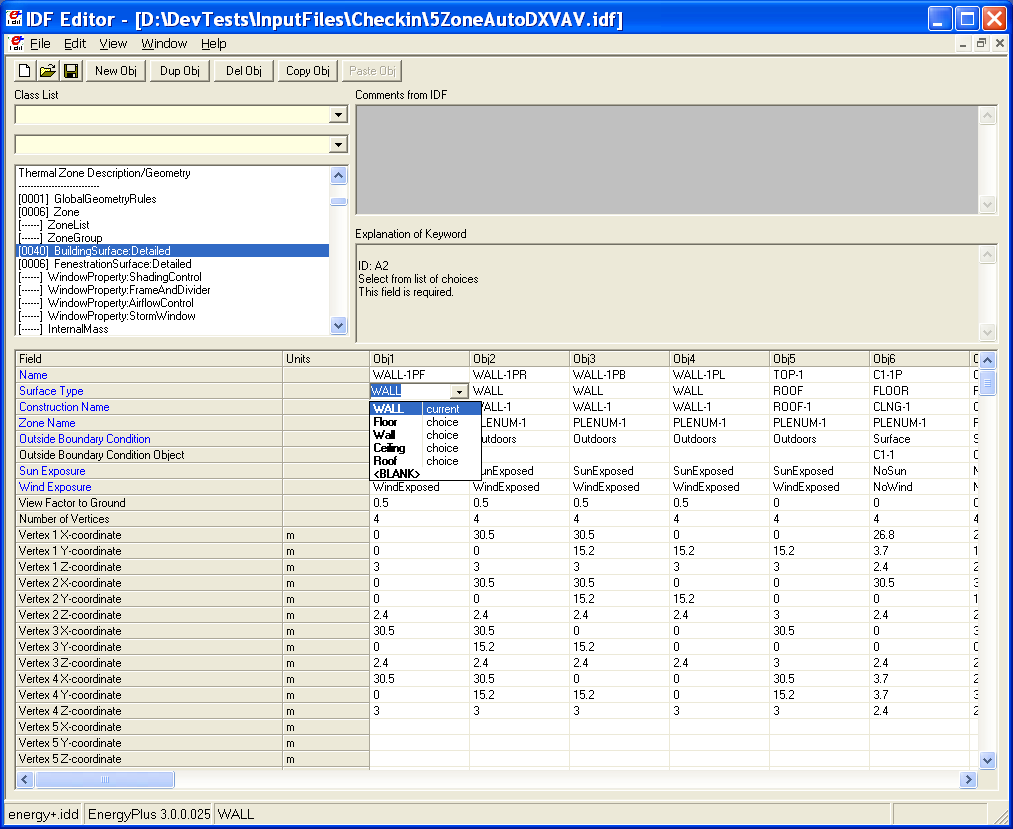
\includegraphics[width=0.9\textwidth, height=0.9\textheight, keepaspectratio=true]{media/image115.png}
\caption{IDF Editor Screen. \protect \label{fig:idf-editor-screen.}}
\end{figure}

\subsection{Start IDF Editor}\label{start-idf-editor}

IDF Editor should be located in the EnergyPlus\textbackslash{}PreProcessor\textbackslash{}IDFEditor directory where you installed EnergyPlus. By double clicking on the IDF Editor icon you will get a screen similar to the one shown above. IDF Editor works in conjunction with the current EnergyPlus Input Data Directory (IDD) file that resides in the directory where EnergyPlus is installed. Another way to start the IDF Editor is from EP-Launch. Multiple IDF files can be opened at once.

\subsection{Creating or Selecting an Input Data File}\label{creating-or-selecting-an-input-data-file}

Creating a new input data file or selecting an existing input data file can be accomplished either through use of the File menu on the menu bar at the top of the screen or through use of the New File icon button or Open File icon button on the tool bar.

\subsection{Class List and Objects}\label{class-list-and-objects}

The classes that can be used to make up an IDF file have been organized into groups as shown in the `Class List' portion of the screen. A class is made up of a group of objects. Select a class from the list by clicking on and highlighting the class. The field to the left of the selected class in the `Class List' will either contain {[}------{]} to indicate that this class has no objects in the IDF file or it will contain a number like {[}0003{]} to indicate the number of times the object currently appears in the IDF file. For example, for the BuildingSurface:Detailed class selected in the screen above under the Thermal Zone Description/Geometry group, there are 40 objects in the IDF file. The details for these 40 objects or any new object that is defined are displayed in columns within the grid. Each object is made up of fields and can be used to further define the object. Any units attached to each field are shown in the second column. You may need to scroll down the `field' list or maximize the application to see all of the fields. Likewise, you may need to scroll to the right of the main grid to see other objects.

Options under the view menu can change how you use the Class List. To display only classes that contain objects select the ``show classes with objects only'' option on the ``View'' menu. You can also toggle this feature on and off with CTRL+L. If the file is empty and has no objects, this toggle does not impact the display.

The ``Show Quick Select Dropdowns'' view menu option adds two new input fields to the main screen. The input fields can be used to go quickly to different classes in the main list of classes. By typing in the top input field, the group that starts with those letters are displayed. After selecting one and pressing the tab button, classes in that group are shown and by typing the first few letters, you can easily select a specific class. Pressing tab again displays that class and it objects. This method allows for quick selection of classes if you remember the group name and class name.

\subsection{Changing Values}\label{changing-values}

By clicking and highlighting a value within an object, several things happen:

\begin{enumerate}
\def\labelenumi{\arabic{enumi})}
\item
  Any user comments from the IDF file will be displayed in the `Comments from IDF' portion of the screen
\item
  Any notes contained in the IDD for this input field will be displayed in the `Explanation of Keyword' portion of the screen
\item
  The value can be edited. Depending on the field, a drop down list may display the default value, maximum and minimum, or other keywords that can be used with the field.
\item
  Numeric fields that can be autosized will include ``autosize'' as a selection in the drop down list.
\item
  Some numeric fields have a maximum and/or minimum value specified in the IDD. If the value entered is outside this range, the cell will be highlighted in pale orange.
\item
  For values that are names of nodes, a new dialog box titled ``Edit or Select Node Name'' can be shown when the small button is pressed that is on the right side in each node name cell as described in the next section.
\end{enumerate}

\subsection{Edit or Select Node Names Dialog}\label{edit-or-select-node-names-dialog}

The following dialog box is displayed when the small button is pressed that is on the right side of cells used for node names. Double clicking on cells containing node names can also make the dialog box appear.

\begin{figure}[hbtp] % fig 50
\centering
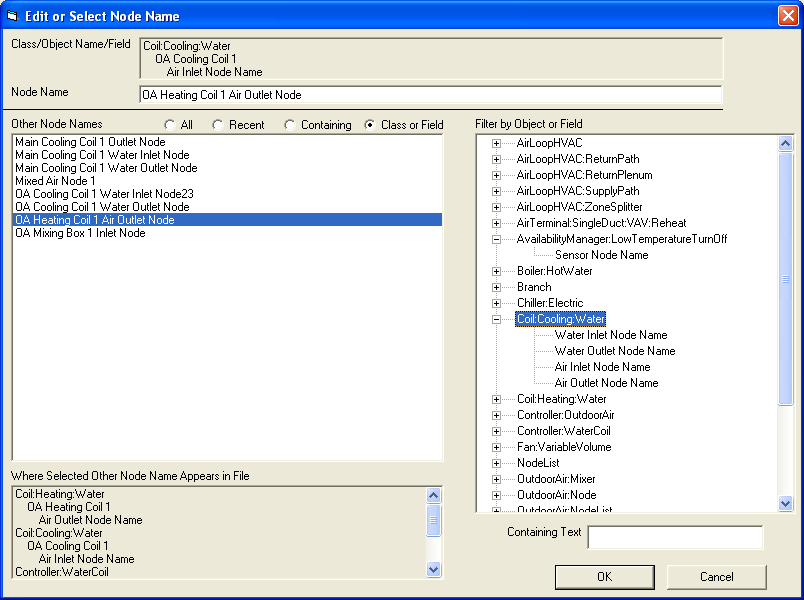
\includegraphics[width=0.9\textwidth, height=0.9\textheight, keepaspectratio=true]{media/image116.png}
\caption{Edit or Select Node Name Dialog Box \protect \label{fig:edit-or-select-node-name-dialog-box}}
\end{figure}

To enter a new node name, type it in the ``Node Name'' field near the top of the dialog. To select a name of a node that is already being used in the file, choose a node name from the list shown on the left of the dialog box and labeled ``Other Node Names.'' When a node name is selected from the list on the left side of the dialog box, the box near the bottom left shown as ``Where Selected Other Node Name Appears in File'' will display the name of the class, name of the object and name of the field for each other location in the file that node name is currently be used.

The Other Node Names list on the left side of the dialog box may contain a very long list of node names depending on the complexity of the HVAC system. To help with this, four options are available just above the list titled All, Recent, Containing, and Class or Field. The All option shows all node names used in the file while the other options are used to narrow the list down to only certain node names. The Recent option shows only node names that have recently been edited. The Containing option shows a list on the right side of the dialog box called ``Filter by Contents'' which shows all of the various words used as part of node names. These words can be selected and the Other Node Names list will only show node names that contain those words. By selecting words from this list, the list of Other Node Names can be shortened very quickly. The last option, Class or Field, shows a hierarchical list on the right side titled Filter by Object or Field containing the list of classes and fields that can have node names. By selecting an object or a field, the Other Node Names list on the right shows only node names that are present in the selected object or field. This is another way of quickly shortening the list of Other Node Names so that the appropriate node name can be selected.

Finally, the Containing Text field just above the OK button can be typed in. Whatever you type limits the Other Node Names list to just those characters. The more typed, the shorter the list becomes. This is another method of quickly finding the node name used in other parts of the file. The Containing Text field is usually used with the All option but can be used with the other display options as well.

\subsection{Working with Objects}\label{working-with-objects}

To delete an object, first click on any value for the object and then click on the ``Del Obj'' button. To add a new object, click on the ``New Obj'' button and a new object column with fields set to blanks, zeros, or default values will be added to the far right of the grid. The ``Dup Obj'' button is similar to ``New Obj'', but copies the values of the fields of the currently selected object. Copying and pasting an object or groups of objects is also possible using the ``Copy Obj'' and ``Paste Obj'' buttons. These allow objects to be copied between files are also good for copying from files in the DataSets subdirectory. (Also see the Edit menu to perform these functions.)

\subsection{File Menu}\label{file-menu-000}

The File menu can be used for creating or selecting input files just like the buttons on the IDF Editor screen (see the \emph{Creating or Selecting an Input File} section above). In addition, the File menu is used to save a file or exit the IDF Editor. More than one file can be opened at a time.

The ``File'', ``Save Options'' screen is shown below.

\begin{figure}[hbtp] % fig 51
\centering
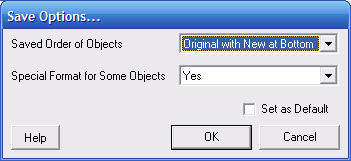
\includegraphics[width=0.9\textwidth, height=0.9\textheight, keepaspectratio=true]{media/image117.png}
\caption{IDF Editor Save Options Screen. \protect \label{fig:idf-editor-save-options-screen.}}
\end{figure}

The save options allow the order of the objects in the file to be sorted by type of object or to keep the original order of the objects (for an existing file). The placement of new objects when the original order is specified can be either at the top or bottom of the file.

In addition, the Save Options also allow certain objects to be written to the file using a specific format that some users prefer.

The settings for the save options are kept for each file saved from the IDF Editor.

The ``Set as Default'' option allows you to keep the save options intact for files that have not been saved yet with a version of IDF Editor that has this capability.

The Help that is available from the Save Options screen is reproduced below:

\begin{itemize}
\item
  The save options are related to the layout of the IDF file after it is saved. These options are not important if you never edit the IDF file with a text editor.
\item
  The sorted order of saving objects is the traditional way the IDF Editor sorts objects within files. Each type of object is presented in groups in the order they appear in the Energy+.IDD. The other options preserve the original order of the objects from the file but each object will be still be reformatted. By preserving the order, the objects are not rearranged so you can group them using a text editor and they will stay in that order. New objects are placed either near the top of the file or near the bottom of the file so that they can be easily found when using a text editor.
\item
  You can also choose to specially format some objects. This affects how individual fields in objects are arranged when saved. Selecting this option will format the following objects on a single line: Report, Report Meter, Report Variable, Version, Timestep in Hour, Inside Convection Algorithm, Outside Convection Algorithm, Solution Algorithm, Shadowing Calculations, Ground Reflectances, and GroundTemperatures:Deep. In addition, Schedule:Compact objects will be formatted to have two field for some lines. With this option, objects with geometric vertices are formatted to have the X, Y, and Z values on the same line. Those objects include: Surface:HeatTransfer, Surface:HeatTransfer:Sub, Surface:Shading:Detached:Fixed, Surface:Shading:Detached:Building and Surface:Shading:Attached.
\item
  These options are saved for each file. If a file has not been saved with IDF Editor yet, the default is used but if a file does not specify the default values for these can also be set by using the set as default option. The saved file keeps these options by using the !-option line with SortedOrder, OriginalOrderTop, OriginalOrderBottom, and UseSpecialFormat."
\item
  Full line comments which begin with ``!'' are preserved by IDF Editor and become associated with the object immediately followin the comment line(s).
\item
  Endline comments which begin with ``!'' are preserved by IDF Editor and are placed immediately before the object they are found in.
\item
  Endline comment which being with ``!-'' are automatic comments which IDF Editor will overwrite with the field name and units. User-provided text which follows ``!-'' will be lost. User comments should be added above the pertinent object using ``!'' to begin the line.
\end{itemize}

Also on the File menu is the Open DataSet menu and submenu. This allows you to open any input file that appears in the DataSet subdirectory and copy objects from them into another file. This is required because EnergyPlus does not read the DataSet files, it is up to you to include objects from them.

\subsection{Edit Menu}\label{edit-menu-000}

The Edit Menu offers options to create a new object, duplicate an object, and delete an object as well as finding and searching. The object options are the same operations as can be accomplished by using the `New Obj', `Dup Obj' and `Del Obj' buttons (see the \emph{Working with Objects} section above). In addition, the ``Next Row after Enter'' option can be toggled. When this option is on, the selection moves down one row after pressing Enter. The copy and paste object commands allow a single object to be copied within a file or between files. The pasted object appears as the last object in the class. This capability makes it easier to utilize the data in the DataSets directory.

The Find Class menu item brings up the following dialog box used to search through the Class List:

\begin{figure}[hbtp] % fig 52
\centering
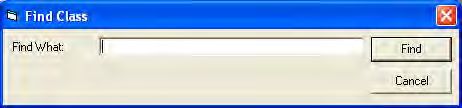
\includegraphics[width=0.9\textwidth, height=0.9\textheight, keepaspectratio=true]{media/image118.png}
\caption{Find Class Dialog Box \protect \label{fig:find-class-dialog-box}}
\end{figure}

The Find Class dialog can be used to find class names quickly and can be activated by the CTRL-F keyboard combination. The Find Previous Class (CTRL-T) and Find Next Class (CTRL-G) can continue the searching process for the next and previous times that the searched text is found in the Class List. If you find this option useful you may also want to try the Show Quick Select Dropdowns option under the View menu which also speeds up searching through the Class List.

The Search and Replace menu item or CTRL-H activates the following dialog box:

\begin{figure}[hbtp] % fig 53
\centering
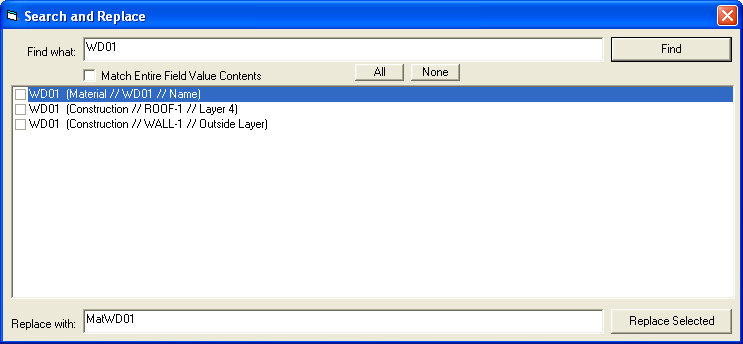
\includegraphics[width=0.9\textwidth, height=0.9\textheight, keepaspectratio=true]{media/image119.png}
\caption{Search and Replace Diaglog Box \protect \label{fig:search-and-replace-diaglog-box}}
\end{figure}

The Search and Replace dialog box can be used to find and change each instance of text being searched with some replacement text. The Search and Replace dialog is used to search and replace values of fields rather than classes like the Find Class dialog. To use the Search and Replace dialog, enter the text being searched in the Find What field and press the Find button. After the Find button is pressed, the list shows the places in the file that the text appears. For each time the text is found, the entire field value is shown followed by the class name, name of the object, and the name of the field in parentheses. Each item in the list can be selected using the check box to the left. The All and None buttons will select all or none of the items found. After the locations are selected that need to be replaced, you should enter the text in the Replace With field. When the Replace Selected button is pressed the value in each of locations that were checked will be replaced with the Replace with text.

The dialog will usually open with the Find What field filled with the value of the currently selected cell. If the current cell has just been changed, the Find What and the Replace With fields will contain the before and after values of the change in the current cell. This makes it easy to change other instances in the file to be consistent with the changes just made. If renaming objects, the recommended approach is to rename the object and select the cell again and open the Search and Replace dialog. This will show other places in the file that use that object name that also may need to be changed.

\subsection{View Menu}\label{view-menu-000}

The View menu offers options for units and column widths. The Narrow/Medium/Wide Column options set the standard column width for items in the object grid. Individual columns can also be resized by dragging the column separator. The displayed value is rounded and/or expressed in scientific notation to fit within the column width.

\begin{enumerate}
\def\labelenumi{\arabic{enumi})}
\item
  EnergyPlus input files are always in SI units. However, selecting ``Inch-Pound'' (IP) units in the View menu displays and edits values in IP units in the IDF editor. The IP unit will be displayed in the units column of the object grid. Some SI units convert to multiple IP units. For example, W becomes Btu/hr for heating and cooling capacity but remains as W for lighting and electrical equipment.
\item
  All conversion factors used in the IDF editor are documented in a block of comments near the top of the Energy+.IDD file.
\item
  Schedules, fluid properties and curves now support IP unit conversions. For curves, the minimum and maximum values are converted but the coefficients are not.
\end{enumerate}

To display only classes that contain objects select the ``show classes with objects only'' option on the ``View'' menu. You can also toggle this feature on and off with CTRL+L. If the file is empty and has no objects, this toggle does not impact the display.

The ``Show Quick Select Dropdowns'' option, which can also be turned on and off with CTRL-Q, displays two dropdown lists above the class list that can be quickly used to select classes. The first list displays the possible groups. Once those are selected, the second list contains only the classes within that group. This option may be used to quickly access classes while avoiding scrolling through the long class list. In addition these pull down menus may be used with the keyboard to select groups and class names based on the first few letters of the names.

The figure below shows the ``Layout Options'' also accessible under the View menu.

\begin{figure}[hbtp] % fig 54
\centering
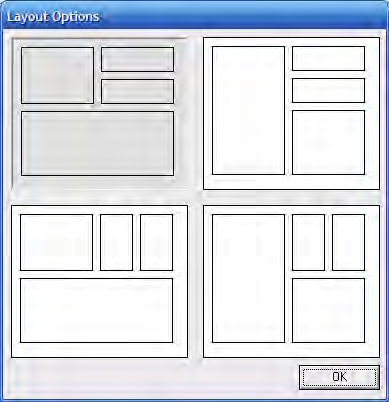
\includegraphics[width=0.9\textwidth, height=0.9\textheight, keepaspectratio=true]{media/image120.png}
\caption{IDF Editor Layout Options Screen. \protect \label{fig:idf-editor-layout-options-screen.}}
\end{figure}

This option allows for different arrangements of the layout for the main screen of the IDF Editor. Select one of the four layouts available.

The ``Show Quick Select Dropdowns'' view menu option adds two new input fields to the main screen. The input fields can be used to go quickly to different classes in the main list of classes.

The ``Validity Check'' function has replaced and expanded upon the old ``Check Out-of-Range'' function. It can also be started by using CTRL-R. The ``Validity Check'' function performs three kinds of validity checks and displays the results as shown in the dialog box below:

\begin{figure}[hbtp] % fig 55
\centering
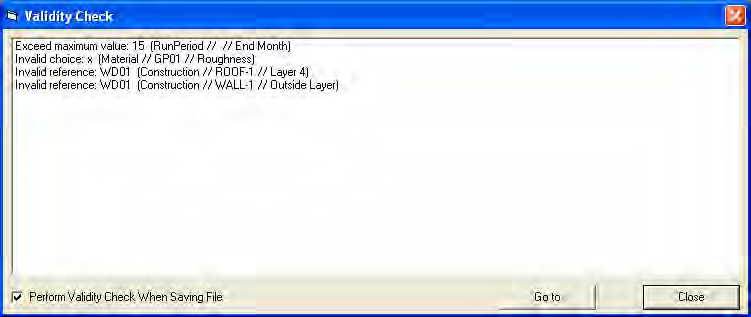
\includegraphics[width=0.9\textwidth, height=0.9\textheight, keepaspectratio=true]{media/image121.png}
\caption{Validity Check Dialog Box \protect \label{fig:validity-check-dialog-box}}
\end{figure}

The list displays the values and locations for objects with values that are either above the maximum or below the minimum values. This allows you to check your input for out-of-range values prior to running EnergyPlus. It also displays fields that contain invalid references. An invalid reference is when a name is used that should be the name of object but no object exists that uses that name. For example, if a Construction object references a layer named IN20 but no Material (or Material:NoMass, etc.) object is named IN20. When viewing the class that contains invalid references, those references are shown with a different background color similar to numbers that are out of range. The ``Validity Check'' dialog also shows when an entry for a field is not one of the possible lists of choices. The Goto button allows you to jump directly to the selected identified problems. The Perform Validity Check When Saving File can be turned on and off and automatically performs the check whenever the file is saved.

\subsection{Help Menu}\label{help-menu-000}

The Help menu offers options to open the EnergyPlus documentation files.

\subsection{Caveats}\label{caveats-000}

Remember to save any changes made before you create or edit another input file.

No ``Run EnergyPlus'' button is available. Save your IDF file and use EP-Launch to execute an EnergyPlus run.

You cannot edit comments in the `Comments from IDF' section of the screen.

The use of point ``.'' or comma ``,'' as the decimal symbol is controlled by the windows system settings. This setting is found in the Control Panel, Regional Options, Number tab, Decimal Symbol field. IDF Editor will use the current decimal symbol to signify the start of the fractional portion of the number and will ignore other symbols. The idf file is always written using point ``.'' as the decimal symbol.

\subsection{Bugs}\label{bugs-000}

Please report any bugs to the helpdesk (email to energyplus-support@gard.com) so that we can fix them prior to the next release.
